%%%%%%%%%%%%%%%%%%%%%%%%%%%%%%%%%%%%%%%%%%%%%%%%%%%%%%%%%%%%%%%%%%%%%%
% writeLaTeX Example: Academic Paper Template
%
% Source: http://www.writelatex.com
% 
% Feel free to distribute this example, but please keep the referral
% to writelatex.com
% 
%%%%%%%%%%%%%%%%%%%%%%%%%%%%%%%%%%%%%%%%%%%%%%%%%%%%%%%%%%%%%%%%%%%%%%
% How to use writeLaTeX: 
%
% You edit the source code here on the left, and the preview on the
% right shows you the result within a few seconds.
%
% Bookmark this page and share the URL with your co-authors. They can
% edit at the same time!
%
% You can upload figures, bibliographies, custom classes and
% styles using the files menu.
%
% If you're new to LaTeX, the wikibook is a great place to start:
% http://en.wikibooks.org/wiki/LaTeX
%
%%%%%%%%%%%%%%%%%%%%%%%%%%%%%%%%%%%%%%%%%%%%%%%%%%%%%%%%%%%%%%%%%%%%%%
\documentclass[twocolumn,showpacs,%
  nofootinbib,aps,superscriptaddress,%
  eqsecnum,prd,notitlepage,showkeys,10pt]{revtex4-1}

\usepackage{amssymb}
\usepackage{amsmath}
\usepackage{graphicx}
\usepackage{dcolumn}
\usepackage{hyperref}
\usepackage{graphicx}
\graphicspath{ {../fig/} }
 
\begin{document}

\title{Predicting Airline Delays: A Comparison of Models and Features}
\author{Dorian Goldman}
\affiliation{Conde Nast, Data Scientist,\\ Columbia University, Adjunct Professor of Data Science\\ }

\begin{abstract}
In this note, we compare different methodologies for predicting airline delays. We focus on all airline delays which are made publicly available on the website of
The Bureau of Transportation Statistics \cite{ontime}. We compare different modeling methodologies including, classification and regression, before and after an enhanced set of features
is introduced. The features which we add to provide supporting predictive accuracy are: weather data from the NOAA \cite{weather}, plane data from the Federal Aviation Administration \cite{aviation}, publicly available holiday data and data about the passenger traffic at USA airports \cite{boarding}. We find
that all three of the above improve predictive performance for regression and classification, with features ranking in the top 10-15 most predictive for the nonlinear models. Motivated by an analysis of the time series, we also implement Poisson regression time series model to predict the mean delay on days and hours prior 
to the day and hour respectively being evaluated. The performance is compared to the standard auto regressive time series model and shown to have significant improvements in the RMSE. The author conjectures that the ideal model would be a contextual Poisson regressive time series, but due to time constraints, this was not implemented. 
\end{abstract}

\maketitle

\section{Introduction}

In this note we briefly summarize the main results obtained in attempting to predict airline delays. We model this problem as 

\begin{equation}
Y^t = f( X_{t-1}) \textrm{ for } t > 0,
\end{equation}

where $t$ is measured in hours, $X_{t-1}$ represents any collection of features we know at time $t-1$ (ie. one hour before the flight) and $f$ is the model we wish to find. 
We believe this is a reasonable assumption in making
in app that would be used to predict delays - expecting to predict delays a day in advance would rely only on general trends of the airline and unreliable weather forecasts, and any probabilistic forecast wouldn't change weather or not an individual needs to be at the airport at the designated time. To be more precise, $X_{t-1}$ represents:
\begin{itemize}
\item Weather data \cite{weather}
\item Plane data \cite{aviation}
\item Holiday data 
\item Airport capacity data \cite{boarding}
\item Time series data on the delays up to time t-1. \cite{airline2}
\end{itemize}
We introduce two time relevant variables based on our exploratory analysis of the distributions of the data each hour and each day. In particular, we consider 
\begin{align} Y_t^{d} &\sim \mathcal{P}(\mu_t^m)\\
Y_t^{h} &\sim \mathcal{P}(\mu_t^h)
\end{align}
where $\mu_t^d = \beta^d \cdot X_{t-1}^d$, $\mu_t^h= \beta^h \cdot X_{t-1}^h$ and $\mathcal{P}$ is a Poisson distribution. We justify this assumption in \cite{airline1} and develop the coefficients in \cite{airline2}.

Our paper is outlined as follows. In Section \ref{sec:main} we discuss the main results of the models with enhanced (all features mentioned above)  and the original variables. We then discuss
the most important features in Subsection \ref{subsec:feats}. We then discuss our methodology in \ref{sub:methodology}.

\section{Discussion of Main Results}
\label{sec:main}

\subsection{Performance}


In this section we display the performance of the models compared. We find that including the features above, our performance improves the ROC by 7-8\% overall. In addition, at least one variable from each dataset above appears in the top 15
features which are most predictive, indicating that each choice of data set did indeed have a meaningful contribution. The comparison of results is summarized in Table \ref{tab:widgets} and the ROC curves are plotted and compared in Figure \ref{fig:ROC}. With more time, the Gradient Boosted Classifier would most likely out perform the Random Forest model, but time wasn't spent on this due to time constraints. 

\begin{table}
\centering
\begin{tabular}{l|r}
Model & AUC\\\hline
Random Forest (Enhanced) & 0.76 \\
Gradient Boosted (Enhanced) & 0.75 \\
Logistic Regr. (Enhanced) & 0.75\\
Random Forest (Original )& 0.70 \\
Gradient Boosted(Original) & 0.70 \\
Logistic Regr. (Original) & 0.65
\end{tabular}
\caption{\label{tab:widgets}Model performance comparison}
\end{table}


\begin{figure}
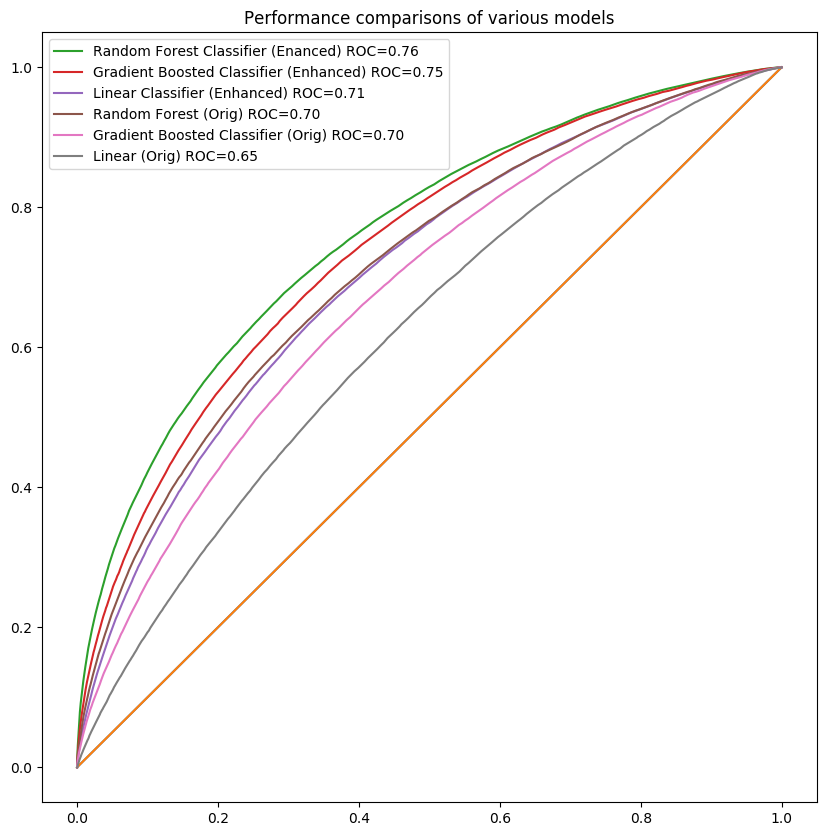
\includegraphics[scale=0.35]{roc_final}
\caption{\label{fig:ROC}ROC Comparison Between Models..}
\end{figure}


\subsection{Most Predictive Features}\label{subsec:feats}

For the reader who wishes to see the feature importance plots for the models with original variables only, we refer to \cite{airline4}. For the enhanced models, we see that features from 4 out of 5 of our original
data sets contribute to the top 15 features. Figure \ref{fig:GB} refers to the Gradient Boosted model and \ref{fig:RF} refers to the Random Forest model. The variables PRCP and SNOW refer respectively to precipitation and snow in mm per hour \cite{weather_readme}, model and issue\_date refer to details of the plane \cite{aviation} and
poisson\_hour and poisson\_day are as defined above, constructed in \cite{airline2}. Finally Holiday.Name is the name of the holiday on any given day. 
\begin{figure}
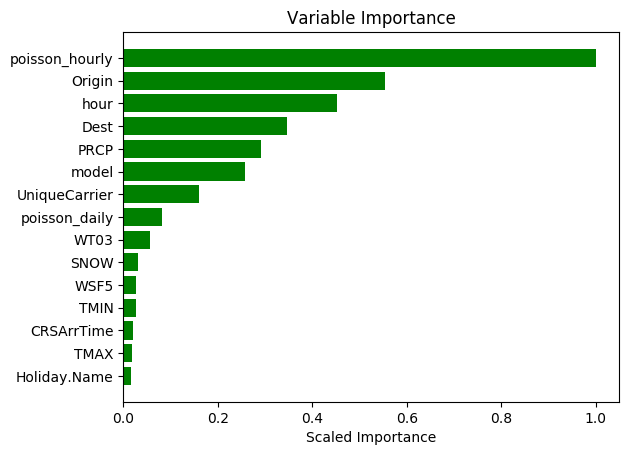
\includegraphics[scale=0.5]{gb_variables}
\caption{\label{fig:GB}GBT Variable Importances.}
\end{figure}

\begin{figure}
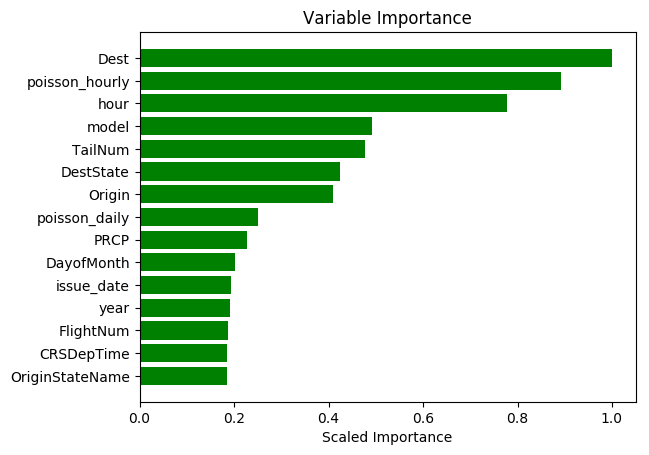
\includegraphics[scale=0.5]{rf_variables}
\caption{\label{fig:RF}RF Variable Importances.}
\end{figure}


\subsection{Methodology}\label{sub:methodology}

We use Python for all of the data processing, and to deal with the very large amount of data (2450509 rows and over 1200 columns when categorical features are expanded), we use the h2o library which performs the model building and analysis in a paralelized way. The work is summarized
in the following notebooks:

\begin{itemize}
\item Airline Delays Part 0 - Processing of Weather Data  \cite{airline1}
\item Airline Delays Part I - Feature Analysis, Preparation and Processing \cite{airline2}
\item Airline Delays Part II - Time Series Analysis \cite{airline3}
\item Airline Delays Part III - Model performance before and after feature enhancement \cite{airline4}
\end{itemize}

For the reader wishing to see the comparison of models, they can safely go to notebook \cite{airline4}. The variables poisson\_hour and poisson\_day are generated in \cite{airline3}. Feature analysis and EDA
which motivate the feature creation and filter out nonsensical values is done in \cite{airline2}. 

% Commands to include a figure:
%\begin{figure}
%\includegraphics[width=\textwidth]{your-figure's-file-name}
%\caption{\label{fig:your-figure}Caption goes here.}
%\end{figure}



\section{Conclusion}

We see by using a wide variety of data sets , utilizing the seasonality of time series and structure of the underlying distribution, we can improve the performance of the model by a significant amount.



  \begin{thebibliography}{1}

  \bibitem{ontime} RITA/BTS. Bureau of Transportation Statistics.. {\em Airline On-Time Performance Data.} \url{https://www.transtats.bts.gov}. 2016

  \bibitem{aviation}  Federal Aviation Administration.  {\em Flight Standards Service - Civil Aviation Registry} \url{http://stat-computing.org/dataexpo/2009/plane-data.csv}. 2009
  \bibitem{weather}  National Centers for Environmental Information. {\em Local Climatological Data.} \url{ https://www.ncdc.noaa.gov/cdo-web/datatools/lcd}. 2016

  \bibitem{boarding} Federal Aviation Administration. {\em Passenger Boardings at Commercial Service Airports. } \url{https://www.faa.gov/airports/planning_capacity/passenger_allcargo_stats/passenger/media/cy14-commercial-service-enplanements.pdf}. 2014
  \bibitem{airline1} Dorian Goldman. {\em Airline Delays Part I - Feature Analysis, Preparation and Processing } \url{https://github.com/doriang102/Airline_Delays/blob/master/analysis/}. 2017
\bibitem{airline2} Dorian Goldman. {\em Airline Delays Part II - Time Series Analysis.ipynb } \url{https://github.com/doriang102/Airline_Delays/blob/master/analysis/}. 2017
\bibitem{airline3} Dorian Goldman. {\em Airline Delays Part III - Model performance before and after feature enrichment } \url{https://github.com/doriang102/Airline_Delays/blob/master/analysis/}. 2017
\bibitem{airline4} Dorian Goldman. {\em Processing of Weather Data} \url{https://github.com/doriang102/Airline_Delays/blob/master/analysis/}. 2017
\bibitem{weather_readme} National Centers for Environmental Information. {\em Readme File For Daily Global Historical Climatology Network} \url{ftp://ftp.ncdc.noaa.gov/pub/data/ghcn/daily/readme.txt}2016

  \end{thebibliography}
  
\end{document}